% Options for packages loaded elsewhere
\PassOptionsToPackage{unicode}{hyperref}
\PassOptionsToPackage{hyphens}{url}
%
\documentclass[
]{book}
\usepackage{amsmath,amssymb}
\usepackage{iftex}
\ifPDFTeX
  \usepackage[T1]{fontenc}
  \usepackage[utf8]{inputenc}
  \usepackage{textcomp} % provide euro and other symbols
\else % if luatex or xetex
  \usepackage{unicode-math} % this also loads fontspec
  \defaultfontfeatures{Scale=MatchLowercase}
  \defaultfontfeatures[\rmfamily]{Ligatures=TeX,Scale=1}
\fi
\usepackage{lmodern}
\ifPDFTeX\else
  % xetex/luatex font selection
\fi
% Use upquote if available, for straight quotes in verbatim environments
\IfFileExists{upquote.sty}{\usepackage{upquote}}{}
\IfFileExists{microtype.sty}{% use microtype if available
  \usepackage[]{microtype}
  \UseMicrotypeSet[protrusion]{basicmath} % disable protrusion for tt fonts
}{}
\makeatletter
\@ifundefined{KOMAClassName}{% if non-KOMA class
  \IfFileExists{parskip.sty}{%
    \usepackage{parskip}
  }{% else
    \setlength{\parindent}{0pt}
    \setlength{\parskip}{6pt plus 2pt minus 1pt}}
}{% if KOMA class
  \KOMAoptions{parskip=half}}
\makeatother
\usepackage{xcolor}
\usepackage{color}
\usepackage{fancyvrb}
\newcommand{\VerbBar}{|}
\newcommand{\VERB}{\Verb[commandchars=\\\{\}]}
\DefineVerbatimEnvironment{Highlighting}{Verbatim}{commandchars=\\\{\}}
% Add ',fontsize=\small' for more characters per line
\usepackage{framed}
\definecolor{shadecolor}{RGB}{248,248,248}
\newenvironment{Shaded}{\begin{snugshade}}{\end{snugshade}}
\newcommand{\AlertTok}[1]{\textcolor[rgb]{0.94,0.16,0.16}{#1}}
\newcommand{\AnnotationTok}[1]{\textcolor[rgb]{0.56,0.35,0.01}{\textbf{\textit{#1}}}}
\newcommand{\AttributeTok}[1]{\textcolor[rgb]{0.13,0.29,0.53}{#1}}
\newcommand{\BaseNTok}[1]{\textcolor[rgb]{0.00,0.00,0.81}{#1}}
\newcommand{\BuiltInTok}[1]{#1}
\newcommand{\CharTok}[1]{\textcolor[rgb]{0.31,0.60,0.02}{#1}}
\newcommand{\CommentTok}[1]{\textcolor[rgb]{0.56,0.35,0.01}{\textit{#1}}}
\newcommand{\CommentVarTok}[1]{\textcolor[rgb]{0.56,0.35,0.01}{\textbf{\textit{#1}}}}
\newcommand{\ConstantTok}[1]{\textcolor[rgb]{0.56,0.35,0.01}{#1}}
\newcommand{\ControlFlowTok}[1]{\textcolor[rgb]{0.13,0.29,0.53}{\textbf{#1}}}
\newcommand{\DataTypeTok}[1]{\textcolor[rgb]{0.13,0.29,0.53}{#1}}
\newcommand{\DecValTok}[1]{\textcolor[rgb]{0.00,0.00,0.81}{#1}}
\newcommand{\DocumentationTok}[1]{\textcolor[rgb]{0.56,0.35,0.01}{\textbf{\textit{#1}}}}
\newcommand{\ErrorTok}[1]{\textcolor[rgb]{0.64,0.00,0.00}{\textbf{#1}}}
\newcommand{\ExtensionTok}[1]{#1}
\newcommand{\FloatTok}[1]{\textcolor[rgb]{0.00,0.00,0.81}{#1}}
\newcommand{\FunctionTok}[1]{\textcolor[rgb]{0.13,0.29,0.53}{\textbf{#1}}}
\newcommand{\ImportTok}[1]{#1}
\newcommand{\InformationTok}[1]{\textcolor[rgb]{0.56,0.35,0.01}{\textbf{\textit{#1}}}}
\newcommand{\KeywordTok}[1]{\textcolor[rgb]{0.13,0.29,0.53}{\textbf{#1}}}
\newcommand{\NormalTok}[1]{#1}
\newcommand{\OperatorTok}[1]{\textcolor[rgb]{0.81,0.36,0.00}{\textbf{#1}}}
\newcommand{\OtherTok}[1]{\textcolor[rgb]{0.56,0.35,0.01}{#1}}
\newcommand{\PreprocessorTok}[1]{\textcolor[rgb]{0.56,0.35,0.01}{\textit{#1}}}
\newcommand{\RegionMarkerTok}[1]{#1}
\newcommand{\SpecialCharTok}[1]{\textcolor[rgb]{0.81,0.36,0.00}{\textbf{#1}}}
\newcommand{\SpecialStringTok}[1]{\textcolor[rgb]{0.31,0.60,0.02}{#1}}
\newcommand{\StringTok}[1]{\textcolor[rgb]{0.31,0.60,0.02}{#1}}
\newcommand{\VariableTok}[1]{\textcolor[rgb]{0.00,0.00,0.00}{#1}}
\newcommand{\VerbatimStringTok}[1]{\textcolor[rgb]{0.31,0.60,0.02}{#1}}
\newcommand{\WarningTok}[1]{\textcolor[rgb]{0.56,0.35,0.01}{\textbf{\textit{#1}}}}
\usepackage{longtable,booktabs,array}
\usepackage{calc} % for calculating minipage widths
% Correct order of tables after \paragraph or \subparagraph
\usepackage{etoolbox}
\makeatletter
\patchcmd\longtable{\par}{\if@noskipsec\mbox{}\fi\par}{}{}
\makeatother
% Allow footnotes in longtable head/foot
\IfFileExists{footnotehyper.sty}{\usepackage{footnotehyper}}{\usepackage{footnote}}
\makesavenoteenv{longtable}
\usepackage{graphicx}
\makeatletter
\newsavebox\pandoc@box
\newcommand*\pandocbounded[1]{% scales image to fit in text height/width
  \sbox\pandoc@box{#1}%
  \Gscale@div\@tempa{\textheight}{\dimexpr\ht\pandoc@box+\dp\pandoc@box\relax}%
  \Gscale@div\@tempb{\linewidth}{\wd\pandoc@box}%
  \ifdim\@tempb\p@<\@tempa\p@\let\@tempa\@tempb\fi% select the smaller of both
  \ifdim\@tempa\p@<\p@\scalebox{\@tempa}{\usebox\pandoc@box}%
  \else\usebox{\pandoc@box}%
  \fi%
}
% Set default figure placement to htbp
\def\fps@figure{htbp}
\makeatother
\setlength{\emergencystretch}{3em} % prevent overfull lines
\providecommand{\tightlist}{%
  \setlength{\itemsep}{0pt}\setlength{\parskip}{0pt}}
\setcounter{secnumdepth}{5}
\usepackage{booktabs}
\usepackage[]{natbib}
\bibliographystyle{plainnat}
\usepackage{bookmark}
\IfFileExists{xurl.sty}{\usepackage{xurl}}{} % add URL line breaks if available
\urlstyle{same}
\hypersetup{
  pdftitle={TerraHidro User Manual},
  pdfauthor={Division of Earth Observation and Geoinformatics - DIOTG},
  hidelinks,
  pdfcreator={LaTeX via pandoc}}

\title{TerraHidro User Manual}
\author{Division of Earth Observation and Geoinformatics - DIOTG}
\date{2025-10-01}

\usepackage{amsthm}
\newtheorem{theorem}{Theorem}[chapter]
\newtheorem{lemma}{Lemma}[chapter]
\newtheorem{corollary}{Corollary}[chapter]
\newtheorem{proposition}{Proposition}[chapter]
\newtheorem{conjecture}{Conjecture}[chapter]
\theoremstyle{definition}
\newtheorem{definition}{Definition}[chapter]
\theoremstyle{definition}
\newtheorem{example}{Example}[chapter]
\theoremstyle{definition}
\newtheorem{exercise}{Exercise}[chapter]
\theoremstyle{definition}
\newtheorem{hypothesis}{Hypothesis}[chapter]
\theoremstyle{remark}
\newtheorem*{remark}{Remark}
\newtheorem*{solution}{Solution}
\begin{document}
\maketitle

{
\setcounter{tocdepth}{1}
\tableofcontents
}
\chapter{Preface}\label{preface}

\url{http://www.dpi.inpe.br/terrahidro/} \textbar{} \href{mailto:sergio.rosim@inpe.br}{\nolinkurl{sergio.rosim@inpe.br}}

TerraHidro Version 5.2.0

Dr.~Sergio Rosim © 20XX-2023

Division of Earth Observation and Geoinformatics - DIOTG

National Institute for Space Research - INPE

São José dos Campos, Brazil

September 25, 2025

Sponsored by:

\pandocbounded{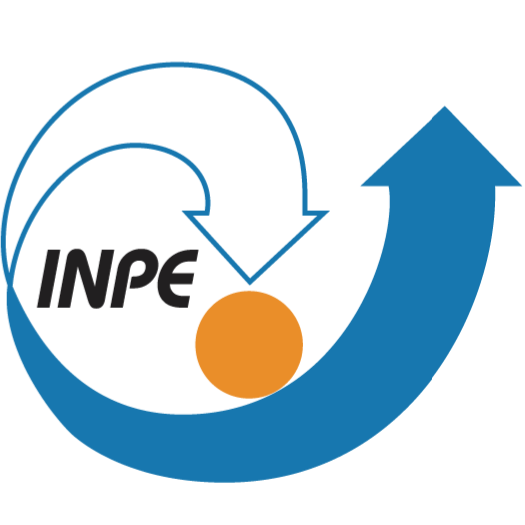
\includegraphics[keepaspectratio]{fig/Inpelogo.png}}

\chapter{Introduction}\label{introduction}

TerraHidro is an advanced geospatial analysis platform designed for hydrological and geomorphometric applications. Developed at the National Institute for Space Research (INPE), it provides a comprehensive suite of tools for digital elevation model (DEM) preprocessing, flow-direction modeling, watershed and stream network delineation, sink removal, floodplain mapping, and terrain analysis. Unlike traditional cartographic or visualization software, TerraHidro serves primarily as an analytical backend, seamlessly integrating with Geographic Information Systems (GIS) such as QGIS.

The system can be used in two main ways:

\begin{itemize}
\item
  QGIS Plugin: For users seeking a graphical workflow, TerraHidro integrates into the QGIS Processing Toolbox, providing intuitive interfaces to execute all functionalities directly within the GIS environment;
\item
  Command-Line Interface (CLI): TerraHidro operates as a stand-alone executable with no installation required. Users can run tools directly from a terminal or incorporate them into automated scripts for large-scale processing.
\end{itemize}

TerraHidro supports raster data in the widely used, e.g.~GeoTIFF format, and provides basic vector operations through ESRI Shapefiles.

By combining high-performance processing with open-source accessibility, TerraHidro enables researchers, students, and professionals to carry out hydrological modeling, geomorphological analysis, and environmental management with precision and reproducibility.

\subsection*{Project Highlights}\label{project-highlights}
\addcontentsline{toc}{subsection}{Project Highlights}

\textbf{Graph-based flow representation} that unifies local flow across digital elevation models;

\textbf{Drainage extraction with pit handling} using methods such as Priority First Search (PFS) to remove spurious depressions and connect flow in flat areas;

\textbf{Large-basin workflows}, with applications demonstrated for Amazon sub-basins;

\textbf{Flexible integration} on TerraLib (C++), with bindings that enable coupling to other hydrological components;

\textbf{Operational efficiency} from graph traversal and storage, supporting scalable accumulation and network operations;

\textbf{Open architecture} that encourages extension and integration in broader GIS environments.

\section*{QGIS Plugin Installation and Setup}\label{qgis-plugin-installation-and-setup}
\addcontentsline{toc}{section}{QGIS Plugin Installation and Setup}

The TerraHidro plugin for the QGIS Processing Toolbox provides users with interfaces that allow all TerraHidro functionalities to be executed directly inside QGIS. However, please note that simply installing the plugin does not guarantee its functionality. It is also necessary to configure an environment variable named \texttt{TERRAHIDRO} that points to the directory where the TerraHidro executable was extracted.

\subsection*{Installing the TerraHidro Plugin in QGIS}\label{installing-the-terrahidro-plugin-in-qgis}
\addcontentsline{toc}{subsection}{Installing the TerraHidro Plugin in QGIS}

\begin{enumerate}
\def\labelenumi{\arabic{enumi}.}
\tightlist
\item
  Open QGIS.\\
\item
  Go to \textbf{Plugins \textgreater{} Manage and Install Plugins\ldots{}}\\
\item
  In the search box, type \textbf{``terrahidro''}.\\
\item
  Select the \textbf{TerraHidro plugin} and click \textbf{Install Plugin}.\\
\item
  Make sure to check the option \textbf{``Show experimental plugins''} under \emph{Options} in the left menu.
\end{enumerate}

\pandocbounded{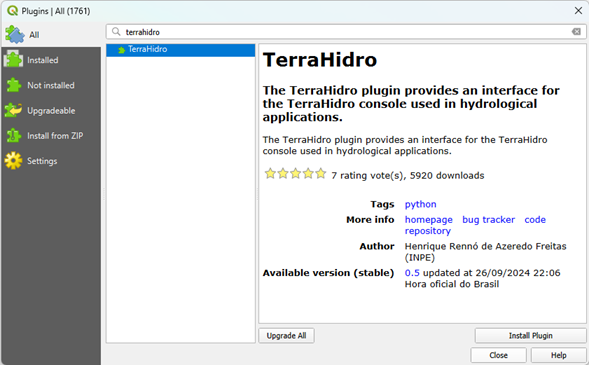
\includegraphics[keepaspectratio]{fig/th_plugin.png}}

After installation, the TerraHidro plugin will appear in the \textbf{Processing Toolbox}.

\pandocbounded{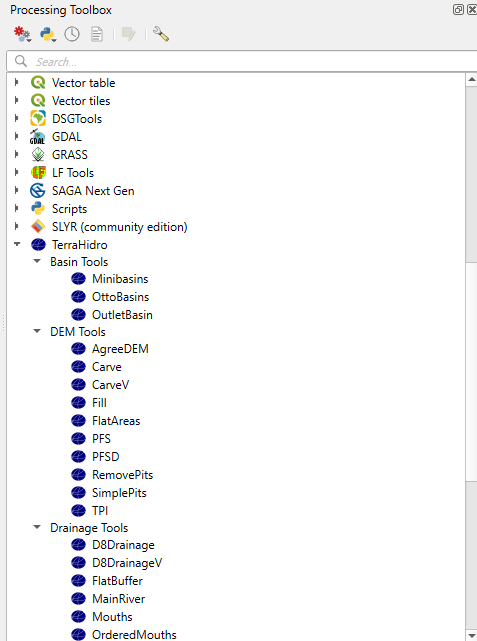
\includegraphics[keepaspectratio]{fig/th_toolbox.png}}

\begin{center}\rule{0.5\linewidth}{0.5pt}\end{center}

\subsection*{\texorpdfstring{Configuring the \texttt{TERRAHIDRO} Environment Variable (Windows)}{Configuring the TERRAHIDRO Environment Variable (Windows)}}\label{configuring-the-terrahidro-environment-variable-windows}
\addcontentsline{toc}{subsection}{Configuring the \texttt{TERRAHIDRO} Environment Variable (Windows)}

In order for the plugin to work properly, you must configure the environment variable \texttt{TERRAHIDRO} to point to the directory where the TerraHidro executable (\texttt{th.exe}) is located. Follow these steps:

\begin{enumerate}
\def\labelenumi{\arabic{enumi}.}
\tightlist
\item
  \textbf{Open the Control Panel}

  \begin{itemize}
  \tightlist
  \item
    Press \textbf{Win + S} to open the search bar.\\
  \item
    Type \textbf{``Control Panel''} and press \textbf{Enter}.
  \end{itemize}
\item
  \textbf{Access Advanced System Settings}

  \begin{itemize}
  \tightlist
  \item
    In the Control Panel, click \textbf{System and Security}.\\
  \item
    Click \textbf{System}.\\
  \item
    On the left panel, click \textbf{Advanced system settings}.
  \end{itemize}
\item
  \textbf{Open Environment Variables}

  \begin{itemize}
  \tightlist
  \item
    In the \emph{System Properties} window, go to the \textbf{Advanced} tab.\\
  \item
    Click the \textbf{Environment Variables\ldots{}} button at the bottom.
  \end{itemize}
\item
  \textbf{Create a New User Variable}

  \begin{itemize}
  \tightlist
  \item
    In the \emph{User variables} section, click \textbf{New}.
  \end{itemize}
\item
  \textbf{Configure the Variable}

  \begin{itemize}
  \tightlist
  \item
    In the \textbf{Variable name} field, type: \texttt{TERRAHIDRO}\\
  \item
    In the \textbf{Variable value} field, type the full path to the directory where the TerraHidro executable is located.

    \begin{itemize}
    \tightlist
    \item
      Example: \texttt{C:\textbackslash{}Users\textbackslash{}\textless{}username\textgreater{}\textbackslash{}Documents\textbackslash{}PROGRAMS\textbackslash{}TerraHidro-5.2.0}
    \end{itemize}
  \end{itemize}
\item
  \textbf{Save and Close}

  \begin{itemize}
  \tightlist
  \item
    Click \textbf{OK} to save the new variable.\\
  \item
    Click \textbf{OK} again to close the \emph{System Properties} window.
  \end{itemize}
\end{enumerate}

\begin{center}\rule{0.5\linewidth}{0.5pt}\end{center}

\subsection*{Final Step}\label{final-step}
\addcontentsline{toc}{subsection}{Final Step}

The \texttt{TERRAHIDRO} environment variable is now configured in your user account, pointing to the directory of the TerraHidro executable. This allows the system to locate and execute TerraHidro from any location in the command prompt or within scripts.

\begin{quote}
\textbf{Important:} Restart any open applications or command prompts so that they recognize the newly created environment variable.
\end{quote}

\section*{Command-Line Interface}\label{command-line-interface}
\addcontentsline{toc}{section}{Command-Line Interface}

TerraHidro can be used directly from the command line, making it a flexible and efficient option for processing terrain and hydrological data. The software is distributed as a stand-alone executable, so no installation is required---just extract the files and call the program from your terminal or command prompt.

Before running any operation, it is important to specify the directory where the TerraHidro executable is located. For example:

We recommend placing both the input and output files in the same directory as the TerraHidro executable. This avoids path errors and ensures that the program can easily locate the required files.

The structure of TerraHidro commands is designed to be simple and intuitive. Most tools follow the general pattern:

\begin{itemize}
\tightlist
\item
  \textbf{\texttt{th}} calls the TerraHidro executable.\\
\item
  \textbf{\texttt{\textless{}operation\textgreater{}}} specifies the tool to be executed (for example, \texttt{d8}, \texttt{removepits}, \texttt{pfs}, \texttt{minibasins}).\\
\item
  \textbf{\texttt{input.tif}} is the input raster file, usually a Digital Elevation Model (DEM).\\
\item
  \textbf{\texttt{output.tif}} is the resulting raster file generated by the operation.
\end{itemize}

For example, to remove pits from a DEM, the command would be:

This straightforward structure makes TerraHidro easy to use while still offering powerful capabilities. By storing all files in the same directory and executing commands step by step, users can build reproducible workflows for DEM preprocessing, flow-direction modeling, watershed delineation, and hydrological hazard simulations.

\subsection*{\texorpdfstring{Example: Removing Pits with the \texttt{pfs} Operation}{Example: Removing Pits with the pfs Operation}}\label{example-removing-pits-with-the-pfs-operation}
\addcontentsline{toc}{subsection}{Example: Removing Pits with the \texttt{pfs} Operation}

The following example demonstrates how to use TerraHidro from the command line:

\begin{Shaded}
\begin{Highlighting}[]
\ExtensionTok{C:\textbackslash{}data}\OperatorTok{\textgreater{}}\NormalTok{th pfs inputDEM.tif outputDEM.tif}
\end{Highlighting}
\end{Shaded}

\begin{itemize}
\tightlist
\item
  \textbf{\texttt{C:\textbackslash{}data\textgreater{}}} indicates the working directory where both the TerraHidro executable (\texttt{th.exe}) and the raster files are stored.\\
\item
  \textbf{\texttt{th}} calls the TerraHidro program.\\
\item
  \textbf{\texttt{pfs}} specifies the operation to be executed. The \emph{Priority-Flood Search (PFS)} algorithm is applied to remove sinks or depressions (pits) from a Digital Elevation Model (DEM), generating a hydrologically consistent surface.\\
\item
  \textbf{\texttt{inputDEM.tif}} is the input raster file containing the original DEM.\\
\item
  \textbf{\texttt{outputDEM.tif}} is the output raster file that will be created, representing the pitless DEM.
\end{itemize}

This simple command ensures that the DEM is corrected for spurious depressions, which is a fundamental preprocessing step before calculating flow directions, contributing areas, and drainage networks.

\begin{quote}
💡 \textbf{Tip -- Changing the Working Directory}

Before running TerraHidro commands, make sure you are in the directory where the executable (\texttt{th.exe}) and your input/output files are located.

On \textbf{Windows}, use the \texttt{cd} command:

\begin{verbatim}
cd C:\Users\<username>\Documents\PROGRAMS\TerraHidro-5.2.0
\end{verbatim}

On \textbf{Linux/MacOS}, use:

\begin{verbatim}
cd /home/<username>/PROGRAMS/TerraHidro-5.2.0
\end{verbatim}

After changing to the correct directory, you can call TerraHidro tools directly, for example:

\begin{verbatim}
th pfs inputDEM.tif outputDEM.tif
\end{verbatim}
\end{quote}

\chapter{Hydrological Analysis}\label{hydrological-analysis}

\section{DEM Pre-processing and Correction}\label{DEM-Pre-processing-and-Correction}

This group of algorithms is designed to transform a raw Digital Elevation Model (DEM) into a hydrologically correct surface where water can flow uninterrupted to the watershed outlet. It addresses common DEM errors like pits (depressions), flat areas, and misalignments with known river networks. The output is a ``pitless'' and ``conditioned'' DEM that is essential for accurate flow direction, watershed delineation, and subsequent hydrological analysis.

\begin{itemize}
\item
  agreedem, carve, carvev, fill, flatareas, pfs, pfsd, removepits, simplepits.
\item
  \hyperref[agreedem]{agreedem}
\item
  \hyperref[carve]{carve}
\item
  \hyperref[carvev]{carvev}
\item
  \hyperref[fill]{fill}
\item
  \hyperref[flatareas]{flatareas}
\item
  \hyperref[pfs]{pfs}
\item
  \hyperref[pfsd]{pfsd}
\item
  \hyperref[removepits]{removepits}
\item
  \hyperref[simplepits]{simplepits.}
\end{itemize}

\subsection{agreedem}\label{agreedem}

\emph{agreedem} modifies a Digital Elevation Model (DEM) to conform to a known drainage network. The tool sharpens the elevation values along the network's cells, effectively burning the channels into the terrain. Users can optionally define a buffer to smooth the elevation of adjacent cells, enhancing the integration of the network with the surrounding topography. This process ensures the DEM's flow directions align with the provided drainage paths.

Input parameters control the sharpening intensity on the network and the degree of smoothing within the specified buffer zone. The tool supports both fixed and variable buffer sizes, which can be defined by an attribute in the input vector data. This operation produces a hydrologically conditioned DEM suitable for subsequent flow routing analysis.

\subsection{carve}\label{carve}

\emph{carve} processes flat areas in a Digital Elevation Model (DEM) by creating an artificial drainage path. The algorithm modifies cell elevations to introduce a slope, enabling hydrological flow routing. It optionally uses a reference drainage network to guide the carving process, ensuring the resulting channel aligns with known flow paths.

The tool requires input parameters to specify whether the drainage network is active (DRNON) and which neighboring cells define a flat area's border (CROSS, DIAG, or ALL). Unlike carvev, which converges carving toward the center of a flat area, carve uses the drainage network to direct the carving trajectory, producing a more accurate hydrological representation.

\emph{See also}: \hyperref[carvev]{carvev}.

\textbf{Parameters}

\begin{longtable}[]{@{}
  >{\raggedright\arraybackslash}p{(\linewidth - 2\tabcolsep) * \real{0.0933}}
  >{\raggedright\arraybackslash}p{(\linewidth - 2\tabcolsep) * \real{0.9067}}@{}}
\toprule\noalign{}
\begin{minipage}[b]{\linewidth}\raggedright
Flag
\end{minipage} & \begin{minipage}[b]{\linewidth}\raggedright
Description
\end{minipage} \\
\midrule\noalign{}
\endhead
\bottomrule\noalign{}
\endlastfoot
\texttt{-i,\ -\/-dem} & Input DEM raster file (e.g., \texttt{inputDEM.tif}). \\
\texttt{-\/-drainage} & Input drainage network (vector \texttt{.shp} or raster), e.g., \texttt{inputDrainage.shp}. \\
\texttt{-\/-flat} & Input flat-areas raster produced by the \emph{flatareas} functionality (e.g., \texttt{inputFlatAreas.tif}). \\
\texttt{-\/-use-drainage} & Defines if the drainage network must be used: • \texttt{DRNON} -- converge ao canal • \texttt{DRNOFF} -- não usa a rede, converge ao centro das planícies (similar ao \texttt{carvev}). \\
\texttt{-\/-border} & Defines which cells form the border of flat areas: • \texttt{CROSS} -- vizinhos horizontais/verticais • \texttt{DIAG} -- vizinhos diagonais • \texttt{ALL} -- todas as direções (8). \\
\texttt{-o,\ -\/-output} & Output DEM raster file with carved flats (e.g., \texttt{outputDEM.tif}). \\
\end{longtable}

\textbf{C++ function}

\begin{Shaded}
\begin{Highlighting}[]
\ExtensionTok{th}\NormalTok{ carve inputDEM.tif inputDrainage.shp inputFlatAreas.tif DRNON}\KeywordTok{|}\ExtensionTok{DRNOFF}\NormalTok{ CROSS}\KeywordTok{|}\ExtensionTok{DIAG}\KeywordTok{|}\ExtensionTok{ALL}\NormalTok{ outputDEM.tif}
\end{Highlighting}
\end{Shaded}

\subsection{carvev}\label{carvev}

\emph{carvev} processes flat areas in a Digital Elevation Model (DEM) by systematically decreasing elevation values from the borders toward the center. This algorithm generates an artificial slope across the feature, forming a characteristic stair-step pattern that enables hydrological flow routing. The operation functions without external drainage data, using only the DEM's own geometry to determine the carving path.

This method provides a foundational correction for hydrologic conditioning. The key distinction from carve is that carvev does not utilize a reference drainage network to guide the process, converging instead on the geometric center of the flat area.

\begin{longtable}[]{@{}
  >{\raggedright\arraybackslash}p{(\linewidth - 2\tabcolsep) * \real{0.2615}}
  >{\raggedright\arraybackslash}p{(\linewidth - 2\tabcolsep) * \real{0.7385}}@{}}
\toprule\noalign{}
\begin{minipage}[b]{\linewidth}\raggedright
Flag
\end{minipage} & \begin{minipage}[b]{\linewidth}\raggedright
Descrição
\end{minipage} \\
\midrule\noalign{}
\endhead
\bottomrule\noalign{}
\endlastfoot
\texttt{-i,\ -\/-dem} & Input DEM raster file \emph{(e.g.,inputDEM.tif)} \\
\texttt{-o,\ -\/-output} & Output DEM raster file with carved flats \emph{(e.g., \texttt{outputDEM.tif})} \\
\end{longtable}

\textbf{C++ function}

\begin{Shaded}
\begin{Highlighting}[]
\ExtensionTok{th}\NormalTok{ carvev inputDEM.tif outputDEM.tif}
\end{Highlighting}
\end{Shaded}

\subsection{fill}\label{fill}

\emph{fill} corrects voids or areas of missing data in a Digital Elevation Model (DEM). The tool uses a separate, often coarser-resolution, reference DEM to supply elevation values for these regions. It replaces null or erroneous cells in the input DEM with corresponding data from the reference source.

This process generates a continuous, hydrologically viable elevation surface. The output DEM supports subsequent terrain analysis by ensuring complete spatial data coverage without interruptions.

\subsection{flatareas}\label{flatareas}

\emph{flatareas} identifies contiguous regions of uniform elevation within a Digital Elevation Model (DEM). The tool scans the input raster for adjacent cells possessing identical elevation values. It then groups these cells into distinct flat features.

The algorithm requires a user-defined minimum area threshold, specified as a number of cells. This parameter excludes smaller, potentially insignificant flat zones from the output. The result is a raster layer where each flat area is classified, providing a basis for subsequent hydrological conditioning procedures.

\subsection{pfs}\label{pfs}

\emph{pfs} removes depressions from a Digital Elevation Model (DEM) using a priority-first search algorithm. The tool initiates a grid search from each pit cell to locate the nearest spill point with a lower elevation. It employs a priority queue to evaluate potential paths, constructing a descending elevation trajectory to the outlet.

This process modifies cell values along the selected path to create a hydrologically continuous surface. The algorithm ensures all depressions are resolved, producing a pit-free DEM suitable for subsequent flow-direction analysis.

\subsection{pfsd}\label{pfsd}

\emph{pfsd} removes depressions from a Digital Elevation Model (DEM) using a priority-first search algorithm that incorporates a reference drainage network. The tool prioritizes the processing of pits located on the drainage network before addressing upstream depressions. It constructs hydrologic outlets by carving descending elevation paths to the nearest lower cell.

This method ensures the resulting drainage structure aligns with the provided network. The algorithm differs from pfs by utilizing the drainage network to guide the depression-removal sequence, enhancing hydrological consistency with known channel locations.

\subsection{removepits}\label{removepits}

\emph{removepits} processes a Digital Elevation Model (DEM) to eliminate hydrological depressions and flat areas. This tool executes a sequence of operations, specifically the carvev, simplepits, and pfs algorithms, to ensure comprehensive hydrological correction. It produces a fully connected drainage surface where water can flow uninterrupted to the watershed outlet.

The procedure first addresses flat regions by carving drainage paths, then removes simple pits through elevation filling, and finally resolves complex depressions via priority-first search. The output is a pit-free DEM suitable for deriving accurate flow direction and accumulation networks.

\subsection{simplepits}\label{simplepits}

\emph{simplepits} processes a Digital Elevation Model (DEM) to remove simple hydrological depressions. The algorithm identifies pit cells with no downstream outlet and elevates them to the lowest value of a neighboring cell plus a minor increment. This adjustment creates a functional drainage path while minimizing alteration to the original topography.

The tool addresses only depressions where this modification does not generate new downstream pits. It serves as an initial processing step for depression removal and is typically followed by more comprehensive algorithms to resolve complex hydrologic discontinuities.

\emph{See also}: \hyperref[removepits]{removepits}.

\textbf{preprocessado} (ex.: \emph{BreachDepressions}) para remover depressões e áreas planas.

\emph{See also}: \hyperref[AverageUpslopeFlowpathLength]{AverageUpslopeFlowpathLength}, \emph{BreachDepressions}.

\textbf{Parameters}

\begin{longtable}[]{@{}ll@{}}
\toprule\noalign{}
Flag & Description \\
\midrule\noalign{}
\endhead
\bottomrule\noalign{}
\endlastfoot
\texttt{-i,\ -\/-dem} & Input raster DEM file \\
\texttt{-o,\ -\/-output} & Output raster file \\
\end{longtable}

\section{Flow Analysis, Drainage Network Extraction and Characterization}\label{Flow-Analysis-Drainage-Network-Extraction-and-Characterization}

\begin{itemize}
\tightlist
\item
  \hyperref[d8]{d8}\\
\item
  \hyperref[d8ca]{d8ca}\\
\item
  \hyperref[d8drainage]{d8drainage}\\
\item
  \hyperref[d8drainagev]{d8drainagev}\\
\item
  \hyperref[segments]{segments}\\
\item
  \hyperref[minibasins]{minibasins}\\
\item
  \hyperref[outletbasin]{outletbasin}\\
\item
  \hyperref[mainriver]{mainriver}\\
\item
  \hyperref[shreve]{shreve}\\
\item
  \hyperref[strahler]{strahler}\\
\item
  \hyperref[ottorivers]{ottorivers}\\
\item
  \hyperref[mouths]{mouths}\\
\item
  \hyperref[orderedmouths]{orderedmouths}
\item
  \hyperref[ottorivers]{ottorivers}
\end{itemize}

\subsection{d8}\label{d8}

\subsection{d8ca}\label{d8ca}

\subsection{d8drainage}\label{d8drainage}

\subsection{d8drainagev}\label{d8drainagev}

\subsection{segments}\label{segments}

\subsection{minibasins}\label{minibasins}

\subsection{outletbasin}\label{outletbasin}

\subsection{mainriver}\label{mainriver}

\subsection{shreve}\label{shreve}

\subsection{strahler}\label{strahler}

\subsection{ottorivers}\label{ottorivers}

\subsection{mouths}\label{mouths}

\subsection{orderedmouths}\label{orderedmouths}

\subsection{ottorivers}\label{ottorivers}

\section{Basin and Sub-basin Delineation}\label{Basin-and-Sub-basin-Delineation}

\begin{itemize}
\tightlist
\item
  \hyperref[minibasins]{minibasins}\\
\item
  \hyperref[outletbasin]{outletbasin}\\
\item
  \hyperref[ottobasins]{ottobasins}
\end{itemize}

\subsection{minibasins}\label{minibasins}

\subsection{outletbasin}\label{outletbasin}

\subsection{ottobasins}\label{ottobasins}

\section{Geomorphometric analysis}\label{Geomorphometric-analysis}

\begin{itemize}
\tightlist
\item
  \hyperref[tpi]{tpi}\\
\item
  \hyperref[hand]{hand}\\
\item
  \hyperref[sand]{sand}\\
\item
  \hyperref[d8slope]{d8slope}
\end{itemize}

\subsection{tpi}\label{tpi}

\subsection{hand}\label{hand}

\subsection{sand}\label{sand}

\subsection{d8slope}\label{d8slope}

\section{Applied Hydrology \& Risk Management}\label{Applied-Hydrology-Risk-Management}

\begin{itemize}
\tightlist
\item
  \hyperref[gfplain]{gfplain}\\
\item
  \hyperref[flowpath]{flowpath}\\
\item
  \hyperref[damcourse]{damcourse}\\
\item
  \hyperref[damsections]{damsections}\\
\item
  \hyperref[dambreak]{dambreak}
\end{itemize}

\subsection{gfplain}\label{gfplain}

\subsection{flowpath}\label{flowpath}

\subsection{damcourse}\label{damcourse}

\subsection{damsections}\label{damsections}

\subsection{dambreak}\label{dambreak}

\chapter{Parts}\label{parts}

You can add parts to organize one or more book chapters together. Parts can be inserted at the top of an .Rmd file, before the first-level chapter heading in that same file.

Add a numbered part: \texttt{\#\ (PART)\ Act\ one\ \{-\}} (followed by \texttt{\#\ A\ chapter})

Add an unnumbered part: \texttt{\#\ (PART\textbackslash{}*)\ Act\ one\ \{-\}} (followed by \texttt{\#\ A\ chapter})

Add an appendix as a special kind of un-numbered part: \texttt{\#\ (APPENDIX)\ Other\ stuff\ \{-\}} (followed by \texttt{\#\ A\ chapter}). Chapters in an appendix are prepended with letters instead of numbers.

\chapter{Footnotes and citations}\label{footnotes-and-citations}

\section{Footnotes}\label{footnotes}

Footnotes are put inside the square brackets after a caret \texttt{\^{}{[}{]}}. Like this one \footnote{This is a footnote.}.

\section{Citations}\label{citations}

Reference items in your bibliography file(s) using \texttt{@key}.

For example, we are using the \textbf{bookdown} package \citep{R-bookdown} (check out the last code chunk in index.Rmd to see how this citation key was added) in this sample book, which was built on top of R Markdown and \textbf{knitr} \citep{xie2015} (this citation was added manually in an external file book.bib).
Note that the \texttt{.bib} files need to be listed in the index.Rmd with the YAML \texttt{bibliography} key.

The RStudio Visual Markdown Editor can also make it easier to insert citations: \url{https://rstudio.github.io/visual-markdown-editing/\#/citations}

\chapter{Blocks}\label{blocks}

\section{Equations}\label{equations}

\begin{itemize}
\tightlist
\item
  \hyperref[AverageFlowpathSlope]{AverageFlowpathSlope}
\item
  \hyperref[AverageUpslopeFlowpathLength]{AverageUpslopeFlowpathLength}
\end{itemize}

\subsection{AverageFlowpathSlope}\label{AverageFlowpathSlope}

Este tool calcula a declividade média (em graus) das rotas de escoamento que passam por cada célula de um DEM.
O DEM deve estar \textbf{preprocessado} (ex.: \emph{BreachDepressions}) para remover depressões e áreas planas.

\emph{See also}: \hyperref[AverageUpslopeFlowpathLength]{AverageUpslopeFlowpathLength}, \hyperref[carve]{carve}.

\textbf{Parameters}

\begin{longtable}[]{@{}ll@{}}
\toprule\noalign{}
Flag & Description \\
\midrule\noalign{}
\endhead
\bottomrule\noalign{}
\endlastfoot
\texttt{-i,\ -\/-dem} & Input raster DEM file \\
\texttt{-o,\ -\/-output} & Output raster file \\
\end{longtable}

\textbf{Python function}

\begin{Shaded}
\begin{Highlighting}[]
\NormalTok{wbt.average\_flowpath\_slope(}
\NormalTok{    dem,}
\NormalTok{    output,}
\NormalTok{    callback}\OperatorTok{=}\NormalTok{default\_callback}
\NormalTok{)}
\end{Highlighting}
\end{Shaded}

\subsection{AverageUpslopeFlowpathLength}\label{AverageUpslopeFlowpathLength}

Identifies and modifies flat areas by decreasing the elevation values from the border to the center.

Here is an equation.

\begin{equation} 
  f\left(k\right) = \binom{n}{k} p^k\left(1-p\right)^{n-k}
  \label{eq:binom}
\end{equation}

You may refer to using \texttt{\textbackslash{}@ref(eq:binom)}, like see Equation \eqref{eq:binom}.

\section{Theorems and proofs}\label{theorems-and-proofs}

Labeled theorems can be referenced in text using \texttt{\textbackslash{}@ref(thm:tri)}, for example, check out this smart theorem \ref{thm:tri}.

\begin{theorem}
\protect\hypertarget{thm:tri}{}\label{thm:tri}For a right triangle, if \(c\) denotes the \emph{length} of the hypotenuse
and \(a\) and \(b\) denote the lengths of the \textbf{other} two sides, we have
\[a^2 + b^2 = c^2\]
\end{theorem}

Read more here \url{https://bookdown.org/yihui/bookdown/markdown-extensions-by-bookdown.html}.

\section{Callout blocks}\label{callout-blocks}

The R Markdown Cookbook provides more help on how to use custom blocks to design your own callouts: \url{https://bookdown.org/yihui/rmarkdown-cookbook/custom-blocks.html}

\chapter{Sharing your book}\label{sharing-your-book}

\section{Publishing}\label{publishing}

HTML books can be published online, see: \url{https://bookdown.org/yihui/bookdown/publishing.html}

\section{404 pages}\label{pages}

By default, users will be directed to a 404 page if they try to access a webpage that cannot be found. If you'd like to customize your 404 page instead of using the default, you may add either a \texttt{\_404.Rmd} or \texttt{\_404.md} file to your project root and use code and/or Markdown syntax.

\section{Metadata for sharing}\label{metadata-for-sharing}

Bookdown HTML books will provide HTML metadata for social sharing on platforms like Twitter, Facebook, and LinkedIn, using information you provide in the \texttt{index.Rmd} YAML. To setup, set the \texttt{url} for your book and the path to your \texttt{cover-image} file. Your book's \texttt{title} and \texttt{description} are also used.

This \texttt{gitbook} uses the same social sharing data across all chapters in your book- all links shared will look the same.

Specify your book's source repository on GitHub using the \texttt{edit} key under the configuration options in the \texttt{\_output.yml} file, which allows users to suggest an edit by linking to a chapter's source file.

Read more about the features of this output format here:

\url{https://pkgs.rstudio.com/bookdown/reference/gitbook.html}

Or use:

\begin{Shaded}
\begin{Highlighting}[]
\NormalTok{?bookdown}\SpecialCharTok{::}\NormalTok{gitbook}
\end{Highlighting}
\end{Shaded}


  \bibliography{book.bib,packages.bib}

\end{document}
